% To generate PDF, type ./run matShrink.tex

\documentclass{article}
\usepackage{arxiv}
\usepackage[numbers]{natbib} % for author-year citation style: \usepackage{natbib}

\usepackage{tablefootnote}

% shortcuts
\newcommand{\WW}[1]{W_\text{#1}}                    % for W_\text{...}
\newcommand{\eR}[2]{$\in \mathbb{R}^{#1 \times #2}$}  % element of R^{1x2}
\newcommand{\mc}[2]{\multicolumn{#1}{c}{#2}}        % table multicolumn
\def\fline{\Xhline{2\arrayrulewidth}}               % fat-line for table

\title{[work in progress]: \\ Matrix-shrink for transformers without loss of accuracy}

\author{Nils Graef\thanks{\texttt{info@openmachine.ai}}, TBD \\
  \href{https://openmachine.ai}{OpenMachine}}

\begin{document} \maketitle

\begin{abstract}
Matrix-shrink reduces the number of weights for back-to-back matrices. It uses matrix inversion to reduce weights in a mathematically equivalent way and thus without compromising model accuracy. Matrix-shrink is applicable to both inference and training. It can be used for inference of existing models without fine-tuning or re-training. We also propose a simplified MLA (multi-head latent attention) scheme. See \citep{tricks} for code and more transformer tricks.
\end{abstract}

For two back-to-back weight matrices $W_A$ and $W_B$, Fig. \ref{fig1} illustrates how we can reduce the size of $W_B$ in a mathematically equivalent way by using matrix inversion.
\begin{figure}[h!] \centering  % the [h!] tries to place the picture right here
  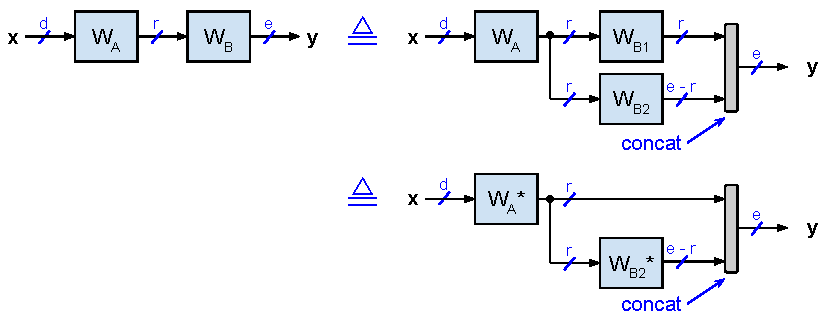
\includegraphics[scale=0.88]{../doc/fig/matShrink_fig1.pdf}
  \caption{Mathematically equivalent implementations of two back-to-back weight matrices $W_A$ and $W_B$ with rank $r$, where $d > r$ and $e > r$. We can split $W_B$ into two submatrices $W_{B1}$ \eR{r}{r} and $W_{B2}$. We can eliminate $W_{B1}$ if it is invertible by merging it into $W_A$ as $W_A^\ast = W_A W_{B1}$ and by changing $W_{B2}$ to $W_{B2}^\ast = W_{B1}^{-1} W_{B2}$. This saves $r^2$ weights and $r^2$ multiply operations per token $x$.}
\label{fig1} \end{figure}

Matrix-shrink reduces the number of weights for the following back-to-back weight matrices:

\begin{itemize}[topsep=-1pt, itemsep=-1pt]
  \item The V and O projections for each attention-head
  \item The Q and K projections for each attention-head (without the RoPE portion)
  \item The latent projections of MLA (multi-head latent attention)
\end{itemize}
\textbf{Related work.} Matrix-shrink is similar to slim attention \citep{slimAttn} in its use of matrix inversion to compute projections from each other. TODO: also mention papers about matrix approximation / compression schemes such as SVD and others.

\textbf{Alternative way.} Alternatively, we can split matrix $W_A$ into two submatrices $W_{A1}$ \eR{r}{r} and $W_{A2}$ such that $W_A = [W_{A1}; W_{A2}]$. We can then eliminate $W_{A1}$ if it is invertible as $W = [W_{A1}; W_{A2}] W_B = [I; W_{A2}^\ast] W_B^\ast$ with identity matrix $I$ \eR{r}{r} and where $W_B^\ast = W_{A1} W_B$ and $W_{A2}^\ast = W_{A2} W_{A1}^{-1}$, see Fig. \ref{fig2}.
\begin{figure}[h!] \centering
  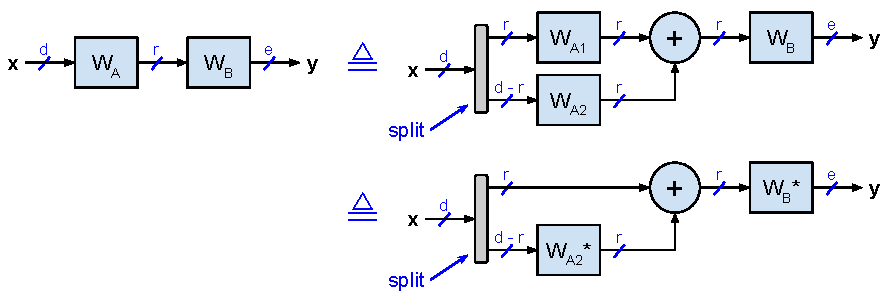
\includegraphics[scale=0.88]{../doc/fig/matShrink_fig2.pdf}
  \caption{Alternative way of shrinking $W_A$ instead of $W_B$}
\label{fig2} \end{figure}

\section{Matrix-shrink for MHA}
Note that the value (V) and output (O) projections for head $i$ of multi-head attention (MHA) are two back-to-back weight matrices $W_{V,i}$ and $W_{O,i}$. Therefore, we can apply the matrix-shrink scheme to each head. Specifically:
\begin{itemize}[topsep=-1pt, itemsep=-1pt]
  \item For the vanilla MHA with $h$ heads, each head has dimension $d_k = d / h$, and $d = d_\text{model}$.
  \item So for the dimensions $r$ and $e$ of Fig. \ref{fig1}, we have  $r = d / h$ and $e = d$.
  \item This saves $r^2 = d^2 / h^2$ weights for each head, so $d^2 / h$ weights in total.
  \item Note: for single-head attention (where $h = 1$), we can save $2 d^2$ weights (i.e. we can merge the V and O weight matrices into a single $d \times d$ matrix; and the Q and K weight matrices into a single $d \times d$ matrix if there is no RoPE).
\end{itemize}

For models that don’t use RoPE (such as Whisper or T5 models), the query (Q) and key (K) projections for each head $i$ of MHA are two back-to-back weight matrices $W_{Q,i}$ and $W_{K,i}$. As with V-O weight matrices, this saves $d^2 / h$ weights.

For many models that use RoPE, we can also apply this trick as follows: Many implementations apply RoPE to only a portion of the head-dimension $d_k = d / h$, usually only to one half of $d_k$. So in this case $r = d_k / 2 = d / (2h)$, which saves only $r^2 = d^2 / (4h^2)$ weights for each head, so $d^2 / (4h)$ weights in total.

\begingroup \renewcommand{\arraystretch}{1.3} % increase table row height by 1.3x
\begin{table}[h!] \centering
\begin{tabular}{lcccccc} \fline
  \thead[l]{Model} & \thead{$d$} & \thead{$d_k$} & \thead{$h$} & \thead{weights \\ $d \times (d_k h)$} & \thead{savings \\ $d_k^2 h$} & \thead{savings \\ \%} \\ \hline
  Whisper-tiny     & 384     & 64    & 6    & 147K    & 25K   & 17\% \\
  CodeGemma-7B     & 3,072   & 256   & 16   & 12.6M   & 1.0M  & 8\%  \\
  T5-3B            & 1,024   & 128   & 32   & 4.2M    & 0.5M  & 12\% \\
  T5-11B           & 1,024   & 128   & 128  & 16.8M   & 2.1M  & 13\% \\ \fline
\end{tabular} \end{table} \endgroup

\section{Matrix-shrink for MLA}
DeepSeek's MLA (multi-head latent attention) scheme \citep{deepseek-v2} has two latent projections, one for Q (queries) and one for KV (keys and values). We can apply matrix-shrink to each of them:
\begin{itemize}[topsep=-1pt, itemsep=-1pt]
  \item The Q-latent projection and query (Q) projections are two back-to-back weight matrices $\WW{DQ}$ and $\WW{UQ}$.
  \item The KV-latent projection and key/value (KV) projections are two back-to-back weight matrices $\WW{DKV}$ and the union of $\WW{UK}$ and $\WW{UV}$.
\end{itemize}
We can also apply matrix-shrink to each V-O head and the non-RoPE portion of the Q-K heads. Specifically, we can apply the matrix-shrink to the MLA weight matrices in the following order:
\begin{enumerate}[topsep=-1pt, itemsep=-1pt]
  \item Apply matrix-shrink to the V-O weight matrices.
  \item Apply matrix-shrink to the NoPE portion (i.e. the non-RoPE portion) of the Q-K weight matrices.
  \item Apply matrix-shrink to the Q-latent projections. This step must be done after applying matrix-shrink to the Q-K weights.
  \item Apply matrix-shrink to the KV-latent projections. This step must be done after applying matrix-shrink to the V-O weights.
\end{enumerate}

Applying matrix-shrink to the KV-latent projections not only reduces weight matrices and corresponding compute, it can also reduce the compute complexity as follows, where $r_\text{KV}$ is the rank of the KV-latent projections.
\begin{itemize}[topsep=-1pt, itemsep=-1pt]
  \item Option 1: Use the $r_\text{KV}$ neurons that don’t require a weight matrix as keys. The number of those keys is $r_\text{KV} / d_\text{NOPE}$. Then these keys can be directly used for the softmax arguments, which saves some computation complexity.
  \item Option 2: Use the $r_\text{KV}$ neurons as values (instead of keys). Then these values can be directly multiplied with the softmax scores, which saves some compute complexity.
\end{itemize}

We are using the following parameter names similar to \citep{deepseek-v2}:
\begin{itemize}[topsep=-1pt, itemsep=-1pt]
  \item For Q (query):
  \begin{itemize}[topsep=-1pt, itemsep=-1pt]
    \item $r_\text{Q}$: rank of Q-latent projection
    \item $\WW{DQ}$: down-projection for Q
    \item $\WW{UQ}$: up-projection for Q-part without RoPE (aka NoPE)
    \item $\WW{QR}$: up-projection for Q-part with RoPE
  \end{itemize}
  \item For KV (key-value):
  \begin{itemize}[topsep=-1pt, itemsep=-1pt]
    \item $r_\text{KV}$: rank of KV-latent projection
    \item $\WW{KR}$: projection for K-part with RoPE (has its own cache, used for all queries as MQA)
    \item $\WW{DKV}$: down-projection for KV
    \item $\WW{UK}$: up-projection for K-part without RoPE (aka NoPE)
    \item $\WW{UV}$: up-projection for V
  \end{itemize}
\end{itemize}

% shortcuts (only letters are allowed in macro names, no numbers and dashes)
\def\dsRone     {\href{https://huggingface.co/deepseek-ai/DeepSeek-R1}         {DeepSeek-R1}}
\def\pplRone    {\href{https://huggingface.co/perplexity-ai/r1-1776}           {R1-1776}}
\def\dsVthree   {\href{https://huggingface.co/deepseek-ai/DeepSeek-V3}         {V3}}
\def\dsVtwoFive {\href{https://huggingface.co/deepseek-ai/DeepSeek-V2.5}       {DeepSeek-V2.5}}
\def\dsVtwoL    {\href{https://huggingface.co/deepseek-ai/DeepSeek-V2-Lite}    {DeepSeek-V2-lite}}
\def\dsVLtwoS   {\href{https://huggingface.co/deepseek-ai/deepseek-vl2-small}  {DeepSeek-VL2-small}}
\def\MiniCPM    {\href{https://huggingface.co/openbmb/MiniCPM3-4B}             {MiniCPM3-4B}}

\begingroup \renewcommand{\arraystretch}{1.3} % increase table row height by 1.3x
\begin{table}[h!] \centering
\begin{tabular}{lcccccccc} \fline
  \thead[l]{Model} & \thead{Params} & $d$ & $r_\text{Q}$ & $r_\text{KV}$ & $h$ & $d_\text{NOPE}$ & $h \cdot d_\text{NOPE}$ & $d_\text{ROPE}$ \\ \hline
  Perplexity \pplRone, \dsRone, and \dsVthree  & 685B  & 7,168  & 1,536  & 512  & 128  & 128  & 16,384  & 64 \\
  \dsVtwoFive                                 & 236B  & 5,120  & 1,536  & 512  & 128  & 128  & 16,384  & 64 \\
  \dsVtwoL, \dsVLtwoS                      & 16B   & 2,048  & N/A    & 512  & 16   & 128  & 2,048   & 64 \\
  OpenBMB \MiniCPM                            & 4B    & 2,560  & 768    & 256  & 40   & 64   & 2,560   & 32 \\ \fline
\end{tabular} \end{table} \endgroup

TODO: add savings to the table above (or a new table)

\section{Simplified MLA}
In this section we propose a simplification for DeepSeek’s MLA (multi-head latent attention).
\begin{figure}[h!] \centering
  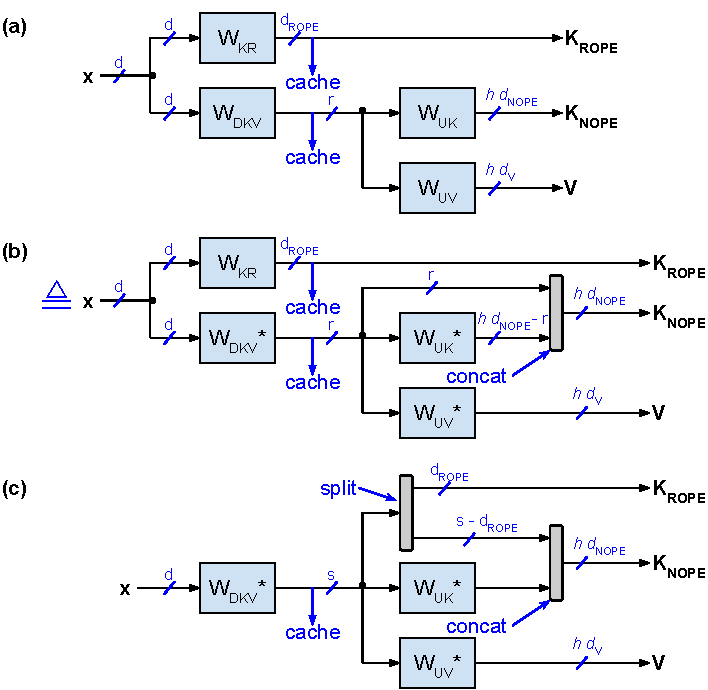
\includegraphics[scale=0.88]{../doc/fig/matShrink_fig3.pdf}
  \caption{K and V projections for MLA. (a) original version; (b) equivalent version optimized by matrix-shrink; (c) proposed simplification}
\label{fig3} \end{figure}

Fig. \ref{fig3} shows the K and V projections of MLA and the proposed simplification:
\begin{itemize}[topsep=-1pt, itemsep=-1pt]
  \item Fig. \ref{fig3}(a) shows the MLA projections for K (keys) and V (values). Note that a single $d_\text{ROPE}$ head is shared among all query-heads, where $d_\text{ROPE} = 64$ or $32$ usually.
  \item Fig. \ref{fig3}(b) shows the mathematically equivalent version with matrix-shrink applied to the weight matrices $\WW{DKV}$ and $\WW{UK}$.
  \item Fig. \ref{fig3}(c) shows the proposed simplified MLA scheme where the $d_\text{ROPE}$ units (or channels) are sourced directly from the latent cache, instead of having a separate cache and $\WW{KR}$:
  \begin{itemize}[topsep=-1pt, itemsep=-1pt]
    \item Note that this simplified scheme is not mathematically identical to the standard MLA scheme shown in Fig. \ref{fig3}(a).
    \item The rank $s$ of the simplified scheme could be larger than $r$ (e.g. $s = r + d_\text{ROPE}$) or slightly lower than this (e.g. $s = r$).
    \item Advantages include: If $s > r$, then there is more usable rank for the keys and values. So the cached latent space is better utilized. And if $s < r + d_\text{ROPE}$ then the total cache size is reduced.
  \end{itemize}
\end{itemize}

\section{Matrix-shrink for GQA and MQA}
Matrix-shrink is not limited to MHA and MLA only. It’s also applicable to GQA (grouped query attention) and MQA (multi-query attention). However, the savings are smaller than for MHA and MLA. Specifically, the savings are reduced by a factor $g$, where $g$ is the number of queries that are shared among a single KV-pair, or in other words $g = n_\text{heads} / n_\text{KV-heads}$ (where $n_\text{heads}$ is the number of query-heads, and $n_\text{KV-heads}$ is the number of KV-heads).

\section{Matrix-shrink for SVD}
In some cases, we can first use SVD (singular value decomposition) to compress the rank of any weight matrix $W$ by a certain percentage. This is applicable for example for the large weight matrices of the transformer’s FFN (feedforward networks). The SVD decomposition factorizes the original matrix $W$ \eR{d}{e} into two matrices $W_A$ and $W_B$ where $r$ is the compressed rank. After performing SVD and compressing the rank by a certain percentage, we can then eliminate $r^2$ weights using our matrix-shrink scheme. Note that reducing the rank by a certain percentage is not an exact implementation of the original matrix $W$ but an approximation.

%\section{Conclusion}
%Slim attention offers a simple trick for halving the context memory of existing MHA transformer models without sacrificing accuracy. Future work includes integrating slim attention into popular frameworks such as HuggingFace Transformers \citep{HFtransformers}, llama.cpp \citep{llama-cpp},  vLLM \citep{vLLM}, llamafile \citep{llamafile}, Ollama \citep{ollama}, SGLang \citep{sglang}, and combining it with existing context memory management schemes such as PagedAttention \citep{pagedAttn} and other compression schemes such as Dynamic Memory Compression DMC \citep{DMC} and VL-cache \citep{VL-cache}.

%\section*{Acknowledgments}
%We would like to thank TBD for helpful feedback on this work.

\bibliographystyle{unsrtnat}
\bibliography{references}

\end{document}
